\documentclass{beamer}
\mode<presentation>


\usepackage[brazil]{babel}
\usepackage[utf8]{inputenc}
 


\usepackage{amsfonts}
\usepackage{amssymb}
\usepackage{amsmath}
\usepackage{algorithm}
\usepackage{algpseudocode}



\usepackage{ae}
\usepackage{graphicx,color}
\usepackage[all]{xy}
\usepackage{empheq}
\usepackage{fancybox}
\usepackage{textcomp}
\usepackage[all]{xy}
\usepackage{textpos}
\usepackage{multicol}
\usepackage{cancel}
\usepackage{listings}
\usepackage{xcolor}
\usepackage{enumerate}
\usepackage{minted}

\usepackage[style=verbose]{biblatex}
\addbibresource{bibtex.bib}

\usepackage{tikz}
\usetikzlibrary{shapes.geometric, arrows}


\tikzstyle{startstop} = [rectangle, rounded corners, minimum width=3cm, minimum 
\tikzstyle{io} = [trapezium, trapezium left angle=70, trapezium right angle=110, minimum width=3cm, minimum height=1cm, text centered, draw=black, fill=blue!30]
\tikzstyle{process} = [rectangle, minimum width=3cm, minimum height=1cm, text centered, draw=black, fill=orange!30]
\tikzstyle{decision} = [diamond, minimum width=3cm, minimum height=1cm, text centered, draw=black, fill=green!30]
\tikzstyle{arrow} = [thick,->,>=stealth]

\newcommand{\floor}[1]{$\lfloor$ #1 $\rfloor$}

\newcommand\Fontvi{\fontsize{9}{7.2}\selectfont}



\usetheme{Boadilla}

\newcommand{\PC}[1]{\ensuremath{\left(#1\right)}}


\newcommand*{\colorboxed}{}
\def\colorboxed#1#{%
  \colorboxedAux{#1}%
}
\newcommand*{\colorboxedAux}[3]{%
  % #1: optional argument for color model
  % #2: color specification
  % #3: formula
  \begingroup
    \colorlet{cb@saved}{.}%
    \color#1{#2}%
    \boxed{%
      \color{cb@saved}%
      #3%
    }%
  \endgroup
}



\title {Pensando Computacionalmente}

\author[Wladimir Araújo Tavares]{ Wladimir Araújo Tavares$^{1}$  }

\institute[UFC]{$^{1}$Universidade Federal do Ceará - Campus de Quixadá\\}
\date{}
\AtBeginSection[]
{
  \begin{frame}<beamer>{}
    \small
    \tableofcontents[currentsection,currentsubsection]
  \end{frame}
}
\begin{document}

\begin{frame}
	\titlepage
\end{frame}

%%%%%%%%%%%%%%%%%%%%%%%%%%%%%%%%%%%%%%%%%%%%%%%%%%%%%%%%%%%%%%%%%%%%



\begin{frame}{Analisando Dados}

\begin{itemize}
\item \textbf{Objetivos:} Desenvolver o pensamento computacional.

\item \textbf{Público-alvo:}  Alunos a partir do primeiro ano do Ensino Médio.

\item \textbf{Conteúdo:} Fluxograma e Análise de Dados

\item \textbf{Tempo:} 50 minutos

\item \textbf{Recursos:} Papel e Caneta

\end{itemize}
    
\end{frame}


% Dois experimentos foram realizados para investigar a dificuldade de fazer a inferência contrapositiva a partir de sentenças condicionais da forma “se P então Q”. Essa inferência,
% que não-P segue de não-Q, requer a transformação da informação apresentada
% na sentença condicional. Sugere-se que a dificuldade se deve a um conjunto mental de
% esperando uma relação de verdade, correspondência ou correspondência entre sentenças e
% estados de coisas. A elicitação da inferência não foi facilitada pela tentativa de
% induzir dois tipos de terapia destinados a quebrar este conjunto. Argumenta-se que os sujeitos
% não deu evidência de ter adquirido as características do “pensamento operacional formal” de Piaget.


\begin{frame}{Passo 1 - Apresentação do Problema}

\begin{itemize}
   
\item <1->Para resolver muitos problemas complexos, precisamos analisar uma grande quantidade de dados. 



\item <2->Considere a seguinte base de dados:

\begin{center}
\begin{tabular}{|l|l|l|}
\hline
M1 & M2 & Resultado\\
\hline
0  & 0 & NC\\
\hline
0  & 1 & NC\\
\hline
1  & 0 & C\\
\hline
1  & 1 & NC\\
\hline
\end{tabular}
\end{center}

M1 representa "Mutação 1'', M2 representa "Mutação 2'', NC representa "Não Câncer" e C representa "Câncer".

\item <3->Utilizando os dados acima, queremos construir um fluxograma para identificar casos de câncer a partir de dados da presença de 2 mutações.

\end{itemize}

\end{frame}


\begin{frame}{Passo 1 - Apresentação da atividade}


\begin{multicols}{2}

\begin{figure}
\begin{center}
	\includegraphics[scale=0.3]{images/data análise.png} 
\end{center}
\caption{Fluxograma para análise para detecção de câncer}
\end{figure}

\columnbreak

\begin{tabular}{|l|l|l|}
\hline
M1 & M2 & Resultado\\
\hline
0  & 0 & NC\\
\hline
0  & 1 & NC\\
\hline
1  & 0 & C\\
\hline
1  & 1 & NC\\
\hline
\end{tabular}





\end{multicols}


 
\end{frame}


% The task is to select those and only those cards that need to be turned over, to
% determine whether the following conditional holds:
% If there is a d on one side,
% then there is a 3 on the other side.

% são quatro pessoas. Podemos ver o que dois deles estão bebendo, mas não quantos anos eles
% está; e podemos ver a idade de dois deles, mas não o que eles estão bebendo: 


% Bob, drinking beer.
% Mary, a senior citizen, obviously over eighteen years old.28
% Computational Logic and Human Thinking
% John, drinking cola.
% Susan, a primary school child, obviously under eighteen years old.
% In contrast with the card version of the selection task, most people solve th

\begin{frame}{Passo 1 - Apresentação da Problemas}

\begin{itemize}

\item Na maioria dos casos, não temos todos os dados disponíveis e precisamos avaliar um grande número de fatores.

\begin{center}
\begin{tabular}{|l|l|l|}
\hline
Idade & Carro & Comprou\\
\hline
20  & M & Sim\\
30  & M & Sim\\
25  & T & Não\\
30  & S & Sim\\
40  & S & Sim\\
20  & T & Não\\
30  & M & Sim\\
25  & M & Sim\\
40  & M & Sim\\
20  & S & Sim\\






\hline

\end{tabular}
\end{center}

M representa "Minivan'', T representa "Truck'' e S representa "Sport" 



 
    

\end{itemize}



\end{frame}


\begin{frame}{Passo 1 - Apresentação da atividade}


\begin{multicols}{2}

\begin{figure}
\begin{center}
	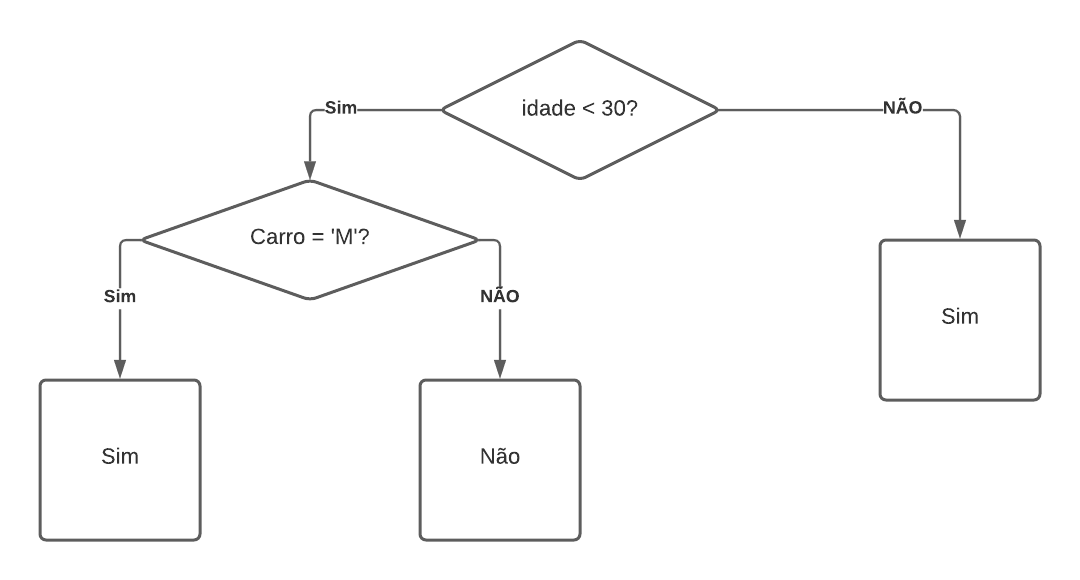
\includegraphics[scale=0.3]{images/carro.png} 
\end{center}

\end{figure}

\columnbreak

\begin{tabular}{|l|l|l|}
\hline
Idade & Carro & Comprou\\
\hline
20  & M & Sim\\
30  & M & Sim\\
25  & T & Não\\
30  & S & Sim\\
40  & S & Sim\\
20  & T & Não\\
30  & M & Sim\\
25  & M & Sim\\
40  & M & Sim\\
20  & S & Sim\\






\hline

\end{tabular}





\end{multicols}


 
\end{frame}

% If a person is drinking alcohol in a bar,
% then the person is at least eighteen years old.

\begin{frame}{Passo 2 - Execução da atividade}

\begin{itemize}

\item <1-> Os alunos devem criar um fluxograma para identificação de casos de câncer a partir dos dados da presença de 5 mutações


\begin{center}
\begin{tabular}{|l|l|l|l|l|l|}
\hline
M1 & M2 & M3 & M4 & M5 & Resultado\\
\hline
0 & 1 & 0 & 1 & 1 & C\\
0 & 0 & 0 & 0 & 0 & NC\\
0 & 0 & 1 & 1 & 0 & NC\\
0 & 0 & 0 & 0 & 0 & NC\\
1 & 1 & 1 & 1 & 1 & C\\
0 & 0 & 0 & 1 & 0 & NC\\
\hline
\end{tabular}
\end{center}

\end{itemize}


\end{frame}


\begin{frame}{Passo 3 - Discussão}

\begin{itemize}

\item <1-> Os alunos devem explicar o processo de criação dos fluxogramas (quais foram os critérios para a escolha das perguntas?).

\item <2-> Refletir sobre os critérios que devem ser considerados para a avaliação dos fluxogramas.

\item <3-> Refletir como avaliar o tempo para utilizar um fluxograma qualquer?

\item <4-> Quantos dados estão faltando na nossa tabela?





\end{itemize}


\end{frame}





\end{document}